\documentclass[aspectratio=1610]{beamer}
\usetheme{boxes}
\usecolortheme{crane}
\usepackage{amsmath,amsfonts}
\usepackage{algpseudocode}
\usepackage{multicol}
\usepackage{pgfplots}
\pgfplotsset{compat=1.15}
\usepackage{mathrsfs}
\usetikzlibrary{arrows}


%-------------------------------------------------------------------
%	 TITLE SLIDE
%-------------------------------------------------------------------


\begin{document}

% -------------------------------------------------------------------
% Lesson 2
% -------------------------------------------------------------------
\section{Software specifications. Formal methods}

\begin{frame}
\begin{center}
\Huge Lesson 2\\~\\
\textbf{Software specifications. Formal methods}
\end{center}
\end{frame}


\begin{frame}
\frametitle{Lesson 2}

\Huge In this lesson we will talk about:
 \alert{Software specifications},
 \alert{Formal methods},
 \alert{Software verification and validation}
\end{frame}



\begin{frame}
\begin{center}
\Huge
\begin{quote}
\textbf{"Todays software has grown by evolution, not by intelligent design"}
\begin{flushright}
{--- Leslie Lamport}	
\end{flushright}
\end{quote}
\end{center}
\end{frame}


\begin{frame}{Lesson 2}{}
\includegraphics[scale=0.30]{Images/loc.png}
\end{frame}


\begin{frame}{Lesson 2}{}
\Huge
 Our software is \textbf{complex}, \textbf{buggy} and \textbf{difficult} to maintain.
 \end{frame}


\begin{frame}
\begin{center}
\Huge
\begin{quote}
\textbf{"If our software is buggy, what does
that say about its security?"}
\begin{flushright}
{--- Prof. Robert H. Morris}
\end{flushright}
\end{quote}
\end{center}
\end{frame}


\begin{frame}[plain,noframenumbering]
\makebox[\linewidth]{\includegraphics[width=\paperwidth]{Images/outage1}}
\end{frame}

\begin{frame}[plain,noframenumbering]
\makebox[\linewidth]{\includegraphics[width=\paperwidth]{Images/outage2}}
\end{frame}

\begin{frame}[plain,noframenumbering]
\makebox[\linewidth]{\includegraphics[width=\paperwidth]{Images/outage3}}
\end{frame}

\begin{frame}{Lesson 2}{}
\Huge
\center
    \textbf{What can we do about it?} 
\end{frame}



\begin{frame}{Lesson 2}{}
\Huge
\begin{center}
   Start with a \textbf{smart design} at the specification level
\end{center}
\end{frame}


\begin{frame}{Lesson 2}{}
\begin{center}
\Huge\textbf{Software Specifications}
\end{center}
\end{frame}


\begin{frame}{Lesson 2}{}
\Huge{What is a specification?}
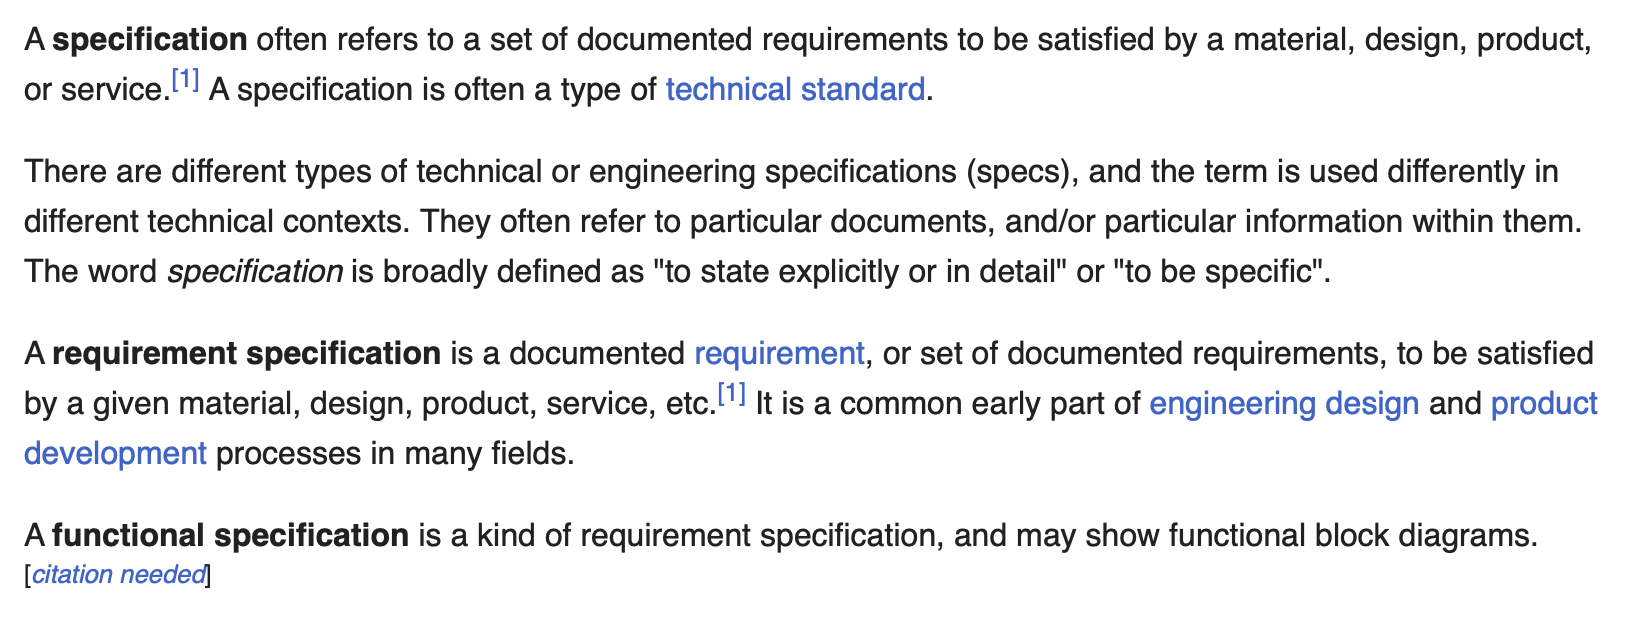
\includegraphics[scale=0.52]{Images/specs}
\end{frame}


\begin{frame}{Lesson 2}{}
\Huge{What is a functional specification?}
\includegraphics[scale=0.46]{Images/funcspecs0}
\end{frame}


\begin{frame}{Lesson 2}{}
\huge
    A \textbf{functional software specification} is a
    \alert{written} description of what our program is supposed to do.
\end{frame}


\begin{frame}{Lesson 2}{}
\includegraphics[scale=0.41]{Images/funcspecs}
\end{frame}



\begin{frame}{Lesson 2}{}
\LARGE
\textbf{How can we write the specification?}\\~\\
\begin{itemize}
    \item English. Finnish. Chinese
    \item Graphical diagrams. Drawing
    \item Technical sketches. Mockups
\end{itemize}
\end{frame}


\begin{frame}{Lesson 2}{}
\LARGE
\textbf{Functional specification}\\~\\
Helps us to understand what our program will do. It’s highly important to write first a specification of our program \alert{before}  implementing and developing anything.
\end{frame}




\begin{frame}{Lesson 2}{}
\LARGE
    \textbf{The specification -- what our program does.}\\~\\
  
\textbf{But how should we describe this specification? How can we be precise? What does it mean to be precise?}
\end{frame}



\begin{frame}{Lesson 2}{}
\begin{center}
\Huge
	Imprecision can lead to \alert{\textbf{ERRORS!}}
\end{center}
\end{frame}


\begin{frame}{Lesson 2}{}
\LARGE
\textbf{Precise specifications}\\~\\
Its difficult to be precise using English or Chinese. Thats why in science and engineering precise specifications have adopted basic maths to describe the specifications.
\end{frame}


\begin{frame}{Lesson 2}{}
\LARGE
\textbf{Basic math}\\~\\
Elementary mathematics. Propositional logic.
\end{frame}


\begin{frame}{Lesson 2}{}
\LARGE
\textbf{Propositional Logic}\\~\\
\includegraphics[scale=0.54]{Images/basiclogic}
\end{frame}


\begin{frame}{Lesson 2}{}
\LARGE
\textbf{Propositional Logic, cont.}
\includegraphics[scale=0.55]{Images/basiclogic2}
\end{frame}



\begin{frame}{Lesson 2}{}
\LARGE
\textbf{Formal methods}\\~\\
\includegraphics[scale=0.53]{Images/fm}
\end{frame}


\begin{frame}{Lesson 2}{}
\LARGE
\textbf{Specifications using formal methods}\\~\\
\includegraphics[scale=0.53]{Images/fms}
\end{frame}


\begin{frame}{Lesson 2}{}
\LARGE
    Formal verification is the use of software tools to prove properties of a formal specification, or to prove that a formal model of a system implementation satisfies its specification.\\~\\
\textbf{Once a formal specification has been developed, the specification may be used as the basis for proving properties of the specification.}
\end{frame}


\begin{frame}{Lesson 2}{}
\LARGE
    \textbf{Verification: Are we building the product right?}

\end{frame}

\begin{frame}{Lesson 2}{}
\LARGE
    \textbf{Validation: Are we building the right product?}
\end{frame}

\begin{frame}{Lesson 2}{}
\LARGE
"Building the product right" checks that the specifications are correctly implemented by the system while "building the right product" refers back to the user's needs. Ideally, formal methods provide a mathematical guarantee that software meets its specifications.
\end{frame}



%\begin{frame}{Lesson 2}{}
%\LARGE
%\textbf{}\\~\\
%A computer system differs from the systems traditionally studied by 
% scientists because we can
%pretend that its state changes in discrete steps. So, we represent the 
%execution
%of a system as a sequence of states. Formally, we define a behavior to be 
%a
%sequence of states, where a state is an assignment of values to 
%variables. We
%specify a system by specifying a set of possible behaviors—the ones 
%representing
%a correct execution of the system

\end{document}

